\chapter*{Dodatak: Prikaz aktivnosti grupe}
		\addcontentsline{toc}{chapter}{Dodatak: Prikaz aktivnosti grupe}
		
		\section*{Dnevnik sastajanja}
		
		\textbf{\textit{Kontinuirano osvježavanje}}\\
		
		 \textit{U ovom dijelu potrebno je redovito osvježavati dnevnik sastajanja prema predlošku.}
		
		\begin{packed_enum}
			\item  sastanak
			
			\item[] \begin{packed_item}
				\item Datum: u ovom formatu: 16. listopada 2023.
				\item Prisustvovali: D.Jenjić, M.Krnić, F.Martinović, L. Matić, J. Rončević, L. Varga, R. Vojinović
				\item Teme sastanka:
				\begin{packed_item}
					\item  međusobno upoznavanje
					\item  prvi sastanak s asistentom i demonstratorom
					\item  rasprava o temi i osnovnim funkcionalnostima 
				\end{packed_item}
			\end{packed_item}
		
			
			\item  sastanak
			\item[] \begin{packed_item}
				\item Datum: u ovom formatu: 25. listopada 2023.
				\item Prisustvovali:  D.Jenjić, M.Krnić, F.Martinović, L. Matić, J. Rončević, L. Varga, R. Vojinović
				\item Teme sastanka:
				\begin{packed_item}
					\item  prva podjela poslova
					\item  rasprava o korištenim tehnologijama
				\end{packed_item}
			\end{packed_item}
			
			\item  sastanak
			\item[] \begin{packed_item}
				\item Datum: u ovom formatu: 29. listopada 2023.
				\item Prisustvovali: D.Jenjić, M.Krnić, F.Martinović, L. Matić, J. Rončević, L. Varga, R. Vojinović
				\item Teme sastanka:
				\begin{packed_item}
					\item  konačna raspodjela dužnosti vezano uz frontend, backend i dokumentaciju
					\item  rasprava o napravljenoj dokumentaciji
				\end{packed_item}
			\end{packed_item}
			
			\vspace{1cm}
			
			\item  sastanak
			\item[] \begin{packed_item}
				\item Datum: u ovom formatu: 30. listopada 2023.
				\item Prisustvovali: D.Jenjić, M.Krnić, F.Martinović, L. Matić, J. Rončević, L. Varga, R. Vojinović
				\item Teme sastanka:
				\begin{packed_item}
					\item  uživo termin s asistentom i demonstratorom
					\item  detaljna rasprava o pojedinim funkcionalnostima aplikacije
					\item  komentiranje napravljenih obrazaca uporabe i sekvencijskih dijagrama
				\end{packed_item}
			\end{packed_item}
			
			\item  sastanak
			\item[] \begin{packed_item}
				\item Datum: u ovom formatu: 14. studenog 2023.
				\item Prisustvovali: D.Jenjić, M.Krnić, F.Martinović, L. Matić, J. Rončević, L. Varga, R. Vojinović
				\item Teme sastanka:
				\begin{packed_item}
					\item  rasprava o dosad napravljenom backendu i frontendu
					\item  rasprava o dijelu dokumentacije koji se tiče baze podataka i ER dijagrama
					\item  dodatna podjela posla unutar frontenda, backenda i dokumentacije
				\end{packed_item}
			\end{packed_item}
			
			
			\item  sastanak
			\item[] \begin{packed_item}
				\item Datum: u ovom formatu: 4. prosinca 2023.
				\item Prisustvovali: D.Jenjić, M.Krnić, F.Martinović, L. Matić, J. Rončević, L. Varga, R. Vojinović
				\item Teme sastanka:
				\begin{packed_item}
					\item  rasprava o poslu vezanom uz implementaciju frontenda i backenda
					\item  podjela posla oko preostale dokumentacije
				\end{packed_item}
			\end{packed_item}
			
			\item  sastanak
			\item[] \begin{packed_item}
				\item Datum: u ovom formatu: 8. siječnja 2024.
				\item Prisustvovali: D.Jenjić, M.Krnić, F.Martinović, L. Matić, J. Rončević, L. Varga, R. Vojinović
				\item Teme sastanka:
				\begin{packed_item}
					\item  rasprava o napravljenom poslu preko praznika
					\item  rasprava o preostalim neostvarenim funkcionalnostima 
					
				\end{packed_item}
			\end{packed_item}
			
			\item  sastanak
			\item[] \begin{packed_item}
				\item Datum: u ovom formatu: 17. siječnja 2024.
				\item Prisustvovali: D.Jenjić, M.Krnić, F.Martinović, L. Matić, J. Rončević, L. Varga, R. Vojinović
				\item Teme sastanka:
				\begin{packed_item}
					\item  podjela preostalog nezavršenog posla pred predaju
					
				\end{packed_item}
			\end{packed_item}
			
			
			
			\item  sastanak
			\item[] \begin{packed_item}
				\item Datum: u ovom formatu: 19. siječnja 2023.
				\item Prisustvovali: D.Jenjić, M.Krnić, F.Martinović, L. Matić, J. Rončević, L. Varga, R. Vojinović
				\item Teme sastanka:
				\begin{packed_item}
					\item  dovršavanje dokumentacije i koda
					\item  ispravljanje grešaka
				\end{packed_item}
			\end{packed_item}
			
			
			%
			
		\end{packed_enum}
		
		\eject
		\section*{Tablica aktivnosti}
		
			\textbf{\textit{Kontinuirano osvježavanje}}\\
			
			 \textit{Napomena: Doprinose u aktivnostima treba navesti u satima po članovima grupe po aktivnosti.}

			\begin{longtblr}[
					label=none,
				]{
					vlines,hlines,
					width = \textwidth,
					colspec={X[7, l]X[1, c]X[1, c]X[1, c]X[1, c]X[1, c]X[1, c]X[1, c]}, 
					vline{1} = {1}{text=\clap{}},
					hline{1} = {1}{text=\clap{}},
					rowhead = 1,
				} 
			
				\SetCell[c=1]{c}{} & \SetCell[c=1]{c}{\rotatebox{90}{\textbf{Matko Krnić}}} & \SetCell[c=1]{c}{\rotatebox{90}{\textbf{Domagoj Jenjić}}} &	\SetCell[c=1]{c}{\rotatebox{90}{\textbf{Filip Martinović}}} & \SetCell[c=1]{c}{\rotatebox{90}{\textbf{Lovro Matić}}} &	\SetCell[c=1]{c}{\rotatebox{90}{\textbf{Jure Rončević}}} & \SetCell[c=1]{c}{\rotatebox{90}{\textbf{Luka Varga}}} &	\SetCell[c=1]{c}{\rotatebox{90}{\textbf{Roko Vojinović}}} \\  
				Upravljanje projektom 		&  10  &  &  &  &  &  \\ 
				Opis projektnog zadatka 	& &  &  &  &  9  &  &  \\ 
				
				Funkcionalni zahtjevi       & 3 &  &  &  &  &  &  \\ 
				Opis pojedinih obrazaca  	& &  &  &  &  3  &  &  \\
				Dijagram obrazaca 			 & 4  &  &  &  & &  7  &  \\
				Sekvencijski dijagrami 		 & &  &  &  &  1  &  & 4  \\
				Opis ostalih zahtjeva 		 &  &  1  &  &  &  &  \\

				Arhitektura i dizajn sustava	  & &  &  &  8 & 2  &  &  \\
				Baza podataka				 & &  &  10  &  &  &  &  \\
				Dijagram razreda 			 &  5  &  &  & & 1 & 2  &  \\
				Dijagram stanja				 &  &  &  &  & 8 &  &  \\
				Dijagram aktivnosti 		 &  &  &  &  & 4 &  &  \\
				Dijagram komponenti			 &  &  &  &  &  &  & 6 & \\ 						
				Korištene tehnologije i alati 		 &  &  &  &  & 1 &  &  \\ 
				Ispitivanje programskog rješenja 	 & 1 &  & 3 &  & 3 &  &  \\
				Dijagram razmještaja			 &  &  &  &  &  &  & 2 & \\
				Upute za puštanje u pogon 		 & 1 &  &  &  & 1 &  &  \\
				Dnevnik sastajanja 			 &  &  &  &  & 3 &  &  \\
				Zaključak i budući rad 		 &  &  &  &  & 1 &  &  \\
				Popis literature 			 &  &  &  &  & 2 &  &  \\
				Implementacija frontenda	 &  &  54  &  &  & 7  & 4 & \\
				Implementacija backenda		 & 13  & 10 & 65  &  &  &  \\
				Deployment					 &  8  &  8  &  &  &  \\
				Izrada početne stranice			  &  &  5  &  &  &  &  \\
				Izrada baze podataka			  &  &  & 10 &  &  &  &  \\
				Dokumentacija					  & 6 &  &  &  & 25 &  &  \\
				
				
			\end{longtblr}
					
					
		\eject
		\section*{Dijagrami pregleda promjena}
		
		\begin{figure}[H]
			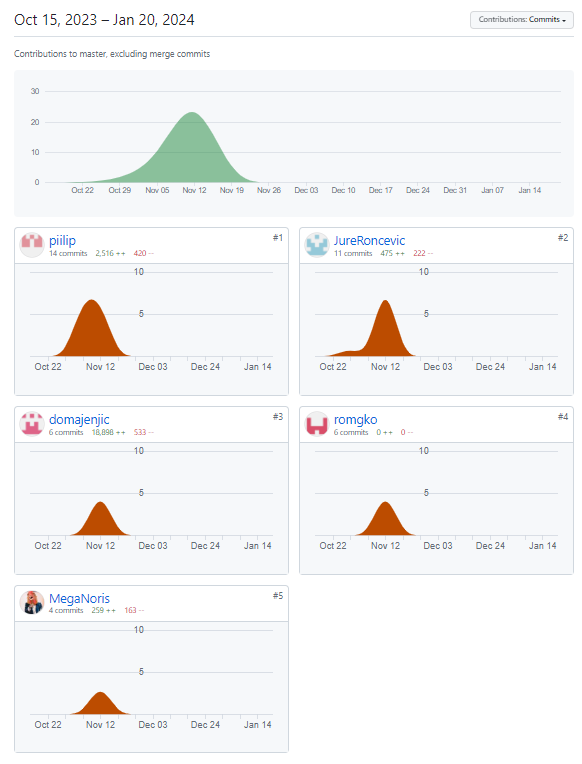
\includegraphics[width=\textwidth]{slike/aktivnost.png} %veličina slike u odnosu na originalnu datoteku i pozicija slike
			\centering
			\caption{Dijagram pregleda promjena}
			\label{fig:dijagramstanja}
		\end{figure}
		
	